%!TEX root = adaptive_dict_kaf.tex

\section{Simulations: Online Operation}

We envision two practical uses of the proposed approach for online time-series prediction: The first one is to determine initial settings for a KAF algorithm (e.g., KLMS), and the second one is to implement the proposed algorithm online using a sliding window. We now show experimental results for these cases using a real-world wind signal from the 2011 PHM Society Conference Data Challenge \cite{windref} and relied on the Python toolbox PyMC3 for maximising or approximating the posterior density.

\subsection{Pre-training for kernel adaptive filters}

We first implemented the proposed method to provide initial conditions for the dictionary, weights, kernel parameter and noise variance for a KLMS algorithm. This aimed to avoid the usual hand-tuning design of KAFs---we refer to this procedure as \emph{pre-training}. The wind data had 2500 samples where the first $270$ samples were used to train our method; we then implemented two KLMS predictors: one with the parameters determined using a maximum-a-posteriori (MAP) fit of the proposed model with fixed dictionary after training, and a standard KLMS with novelty sparsification criterion. For standard KLMS, the novelty criterion parameters were set to have the same number of centres as the proposed model; this is to validate the ability of our method to generate sparse dictionaries against the KLMS, which simply populates the dictionary from the observations.

In both cases the order of the filter was set to $d=5$ and the learning rate was adjusted in each experiment so as to minimise the mean square error (MSE), defined by
\begin{equation*}
\text{MSE} = \frac{1}{n}\sum_{i=1}^{N}\left(y_i - \hat{y}_i\right)^2
\end{equation*}
where $\hat{y}_i$ corresponds to the prediction of the observation $y_i$. 

In order to set the number of centres for pre-training KLMS, we compared different dictionary sizes to assess whether sparsity is achieved independent from the dictionary size. Fig. \ref{wind-confmats} shows the Gram matrices after optimisation of the log-posterior for different choices of dictionary sizes, where it can be seen that the method produces sparse dictionaries for all these choices. We then chose $25$ centres to ensure a sufficiently-rich dictionary, as well as to avoid the increased computational complexity associated by larger dictionaries. Notice that this is the opposite to what we usually do in standard KLMS, where more dictionary elements are needed to compensate for the redundant information that exists among the centres.

%While it may seem that the choice for the dictionary size is somewhat arbitrary given that offline optimisation can induce sparsity on dictionaries of almost any size (see Figure \ref{wind-confmats}), it serves two purposes. 

% Firstly, to be a point of comparison between pre-trained and standard KLMS, and see how same-sized dictionaries can differ when one is restricted to observations only. 

%Secondly, to show that while in KLMS it is natural to think that the more elements in the dictionary, the more it can overcome redundant information that may appear from the chosen centers; pre-training follows an opposite view, in which it is encouraged to choose small sized dictionaries from the start as the optimisation will almost always find a good combination of weights that can generalise the model while preserving sparsity of its elements, with the additional benefit of taking less time to compute because of the reduced dimensionality of the model.

Fig. \ref{wind-series} shows both pre-trained KLMS and standard KLMS side by side, where the shaded area indicates the data used for pre-training. We can see that even though standard KLMS can achieve adequate performance over time, it was outperformed by the proposed pre-trained KLMS in MSE terms---{MSE was calculated after sample 270}. Furthermore, from Fig. \ref{wind-confmat} notice that the final dictionary obtained by pre-trained KLMS is much more sparse than that of standard KLMS due to the proposed sparsity-inducing prior in eq. \eqref{eq:dict_prior}, where taking the centres directly from the more than $2500$ observations resulted in centres that are too close to one another in standard KLMS.

An important finding is that, 
even though KAF methods are typically sensible to the learning rate, we found that our method is much more flexible, since desirable weights were already learned, and as such, the KLMS phase only needs a small learning rate to correct small parameter discrepancies.
\begin{figure}[t!]
	\centering
	\subfloat[]{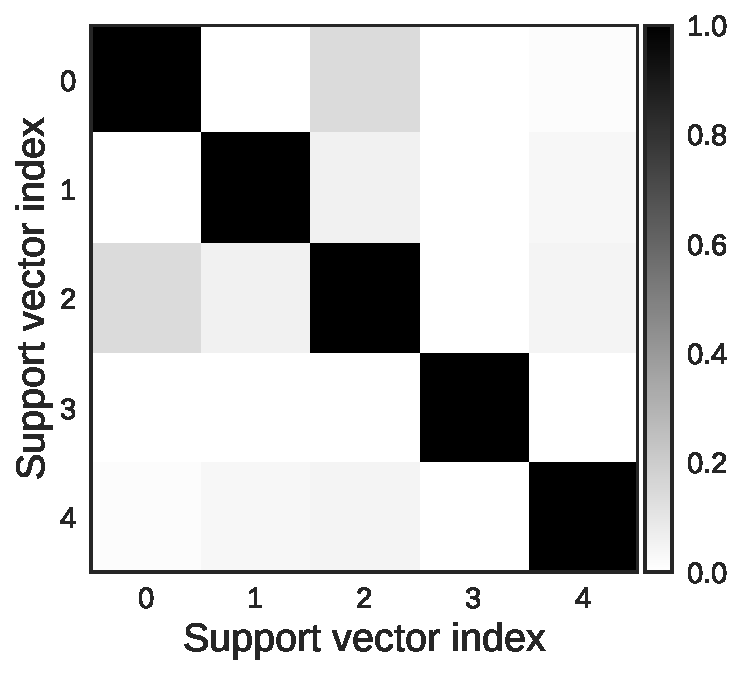
\includegraphics[width=0.165\textwidth]{img/Gram_Wind_Simple_5_2.pdf}}
	\subfloat[]{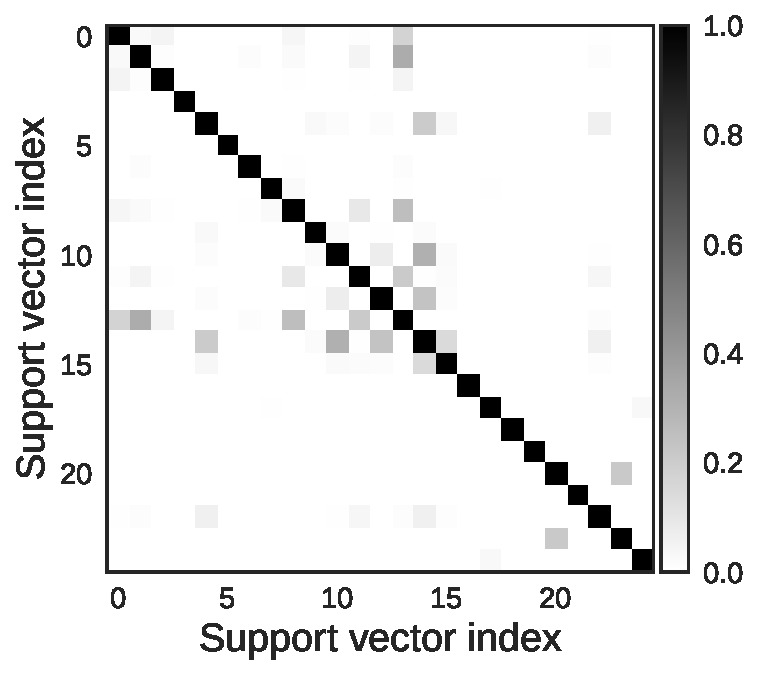
\includegraphics[width=0.17\textwidth]{img/Gram_Wind_Simple_25_2.pdf}}
	\subfloat[]{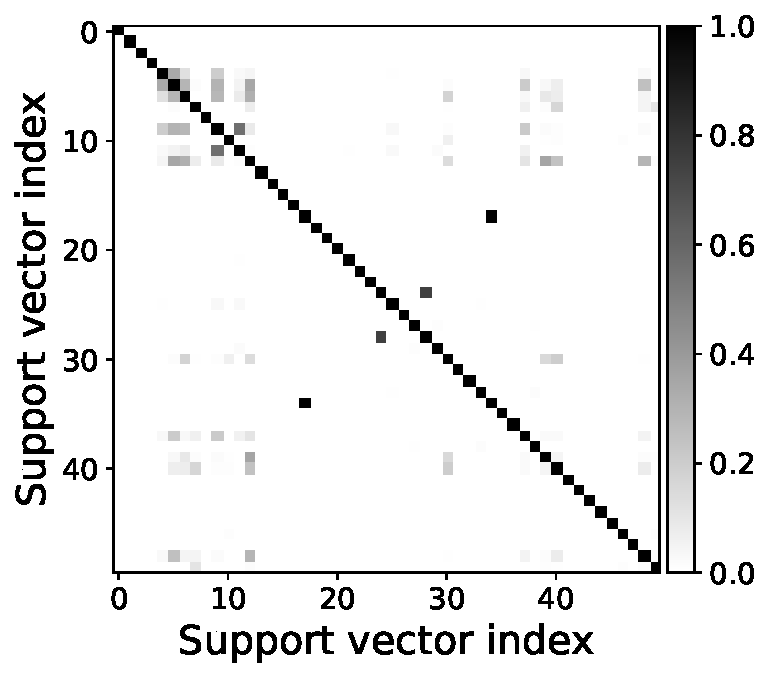
\includegraphics[width=0.17\textwidth]{img/Gram_Wind_Simple_50_2.pdf}}
	\caption{Gram matrices of pre-trained KLMS for wind signals using dictionaries of sizes 5, 25 and 50 (from left to right). In all cases the Gram matrix is close-to-diagonal due to the sparsity-inducing prior.}
	\label{wind-confmats}
\end{figure}

\begin{figure}[t!]
	\centering
	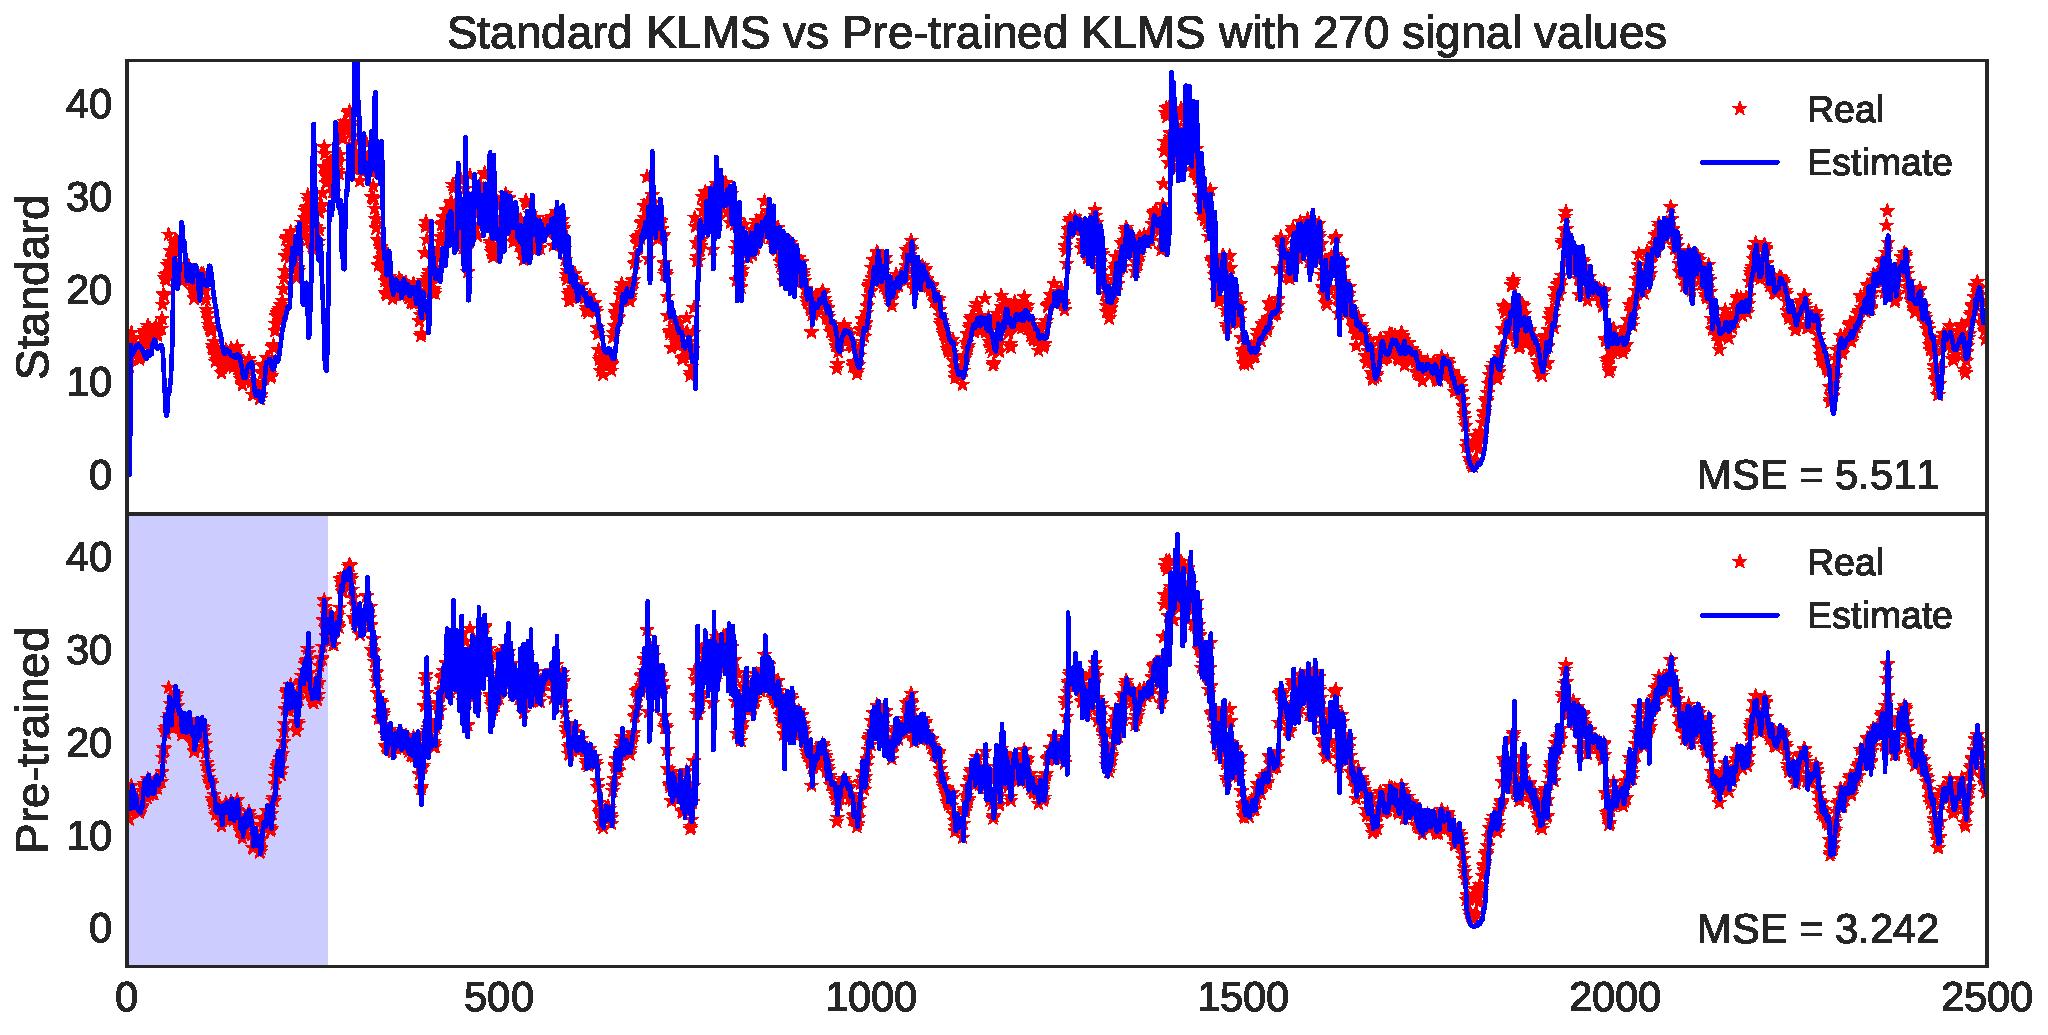
\includegraphics[width=0.5\textwidth]{img/Wind_Offline2.pdf}
	\caption{Wind series estimation: Standard KLMS (top) versus the proposed pre-trained KLMS with 270 training samples (bottom). Shaded area indicates training period and MSE was computed after the 270 time index for a fair comparison.}
	\label{wind-series}
\end{figure}

\begin{figure}[t!]
	\centering
	\subfloat[]{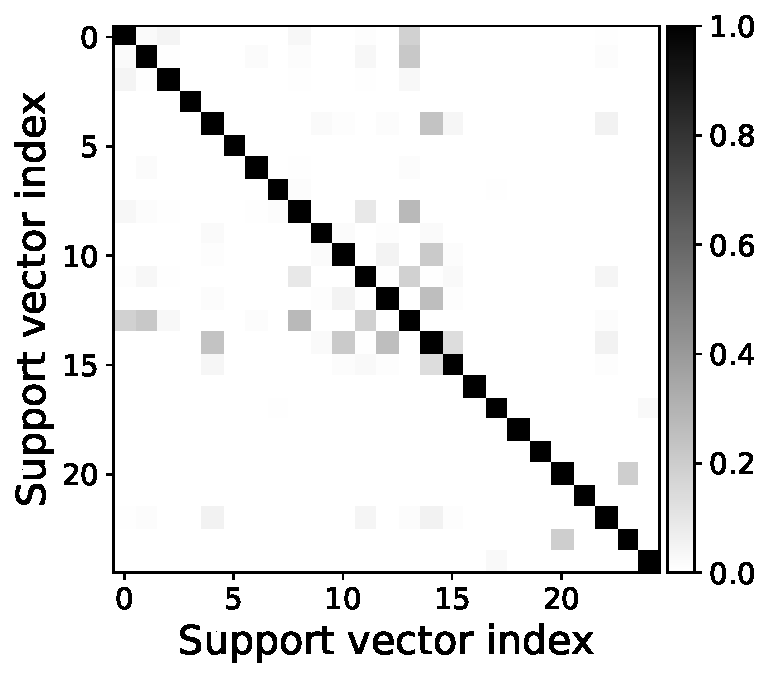
\includegraphics[width=0.17\textwidth]{img/Gram_Wind_pretrained_25.pdf}}
	\subfloat[]{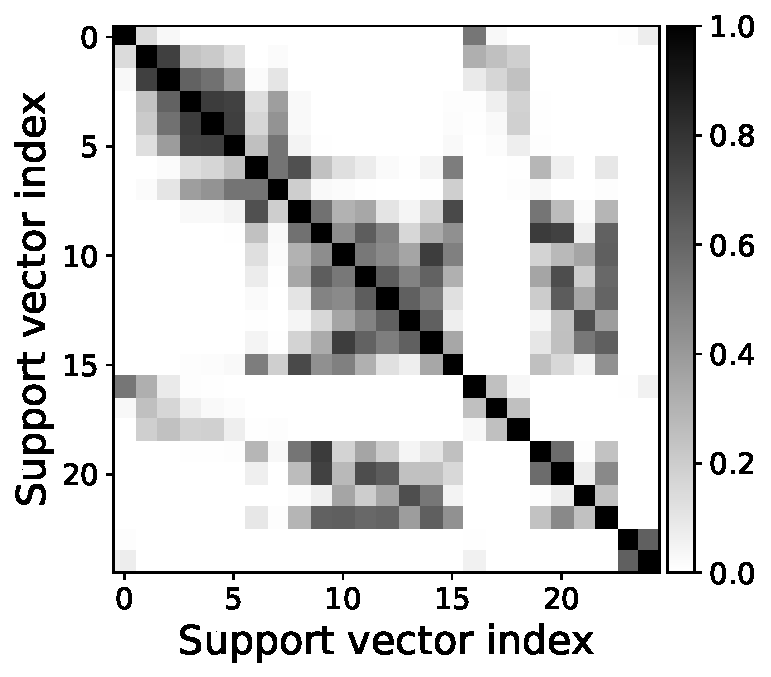
\includegraphics[width=0.17\textwidth]{img/Gram_Wind_standard_25.pdf}}
	\caption{Gram matrices of the pre-trained (left) and standard (right) KLMS dictionaries for wind signals. The proposed pre-trained KLMS yields a much more sparse dictionary than standard KLMS evidenced by a close-to-diagonal Gram matrix. }
	\label{wind-confmat}
\end{figure}


\subsection{Fully-adaptive kernel adaptive filtering}

The second experiment is an online implementation of the proposed model using a sliding window. Specifically, we trained the model sequentially by (i) finding the maximum-a-posteriori (MAP) parameters  in each window, and then (ii) averaging them in time. Denoting $\theta_n^{\text{window}}$ the MAP parameters using data from the $n^\text{th}$ window, the online parameter estimate can be computed by $\theta_{n}^{\text{online}}$ according to
\begin{align}
\theta^{\text{online}}_{1} &= \theta^{\text{window}}_{1}\\ 
\theta_{n}^{\text{online}} &= \rho\theta_n^{\text{window}} + (1-\rho)\theta_{n-1}^{\text{online}}
\end{align}
where $\rho\in(0,1)$ is a forgetting factor balancing confidence between past parameter values and the new estimate. This resembles the kernel recursive least squares (KRLS) \cite{engel04,van2012kernel} rationale but rather than moving the parameters against the gradient as in KRLS, we are moving towards the MAP parameters of the current window. 

\begin{figure}[t!]
	\centering
	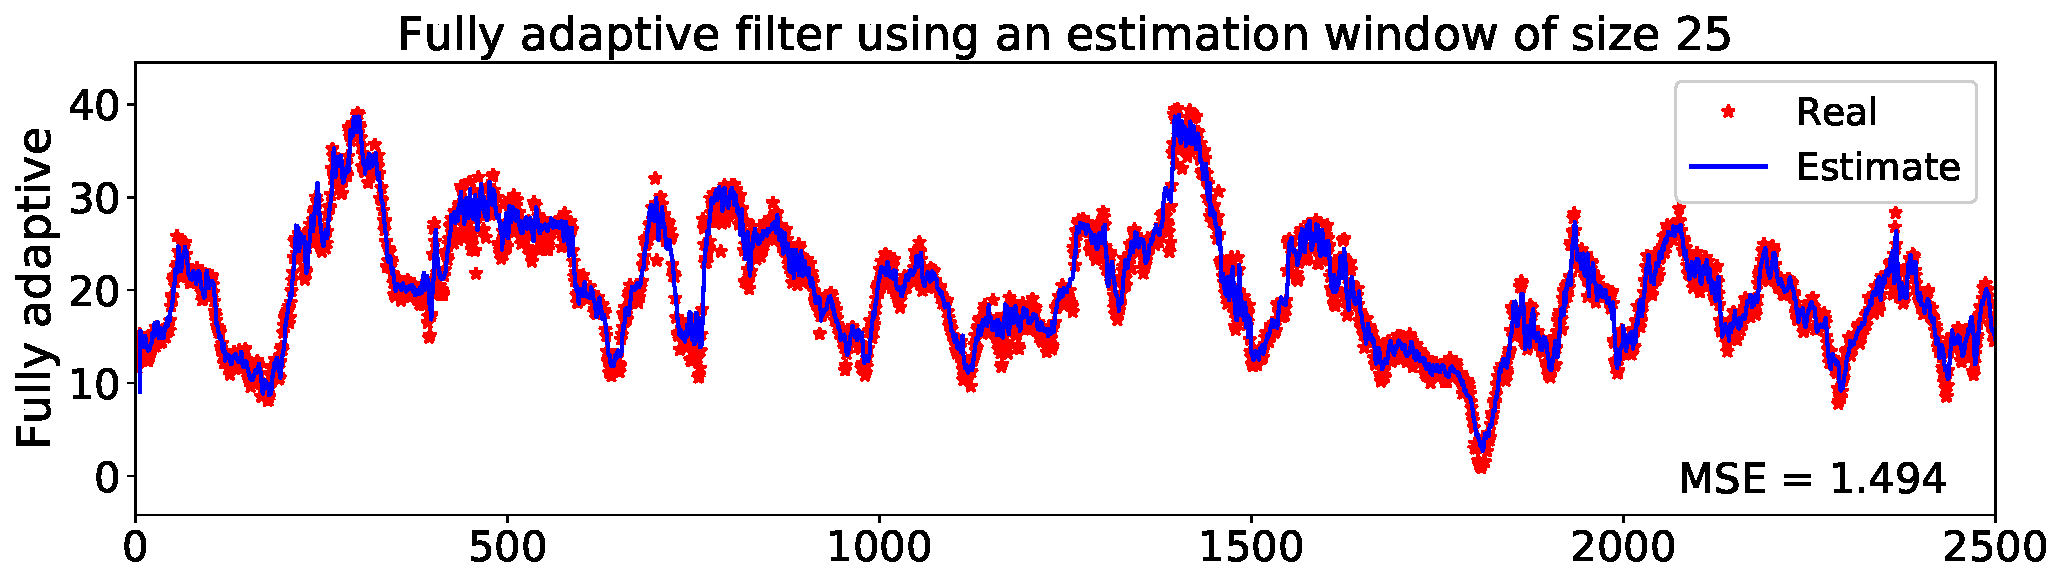
\includegraphics[width=0.5\textwidth]{img/fully_adaptive_estimate3}
	\caption{Fully-adaptive KAF applied to the wind series using a sliding window.}
	\label{fig:adaptive-wind}
\end{figure}

%\begin{figure}[t!]
%	\centering
%	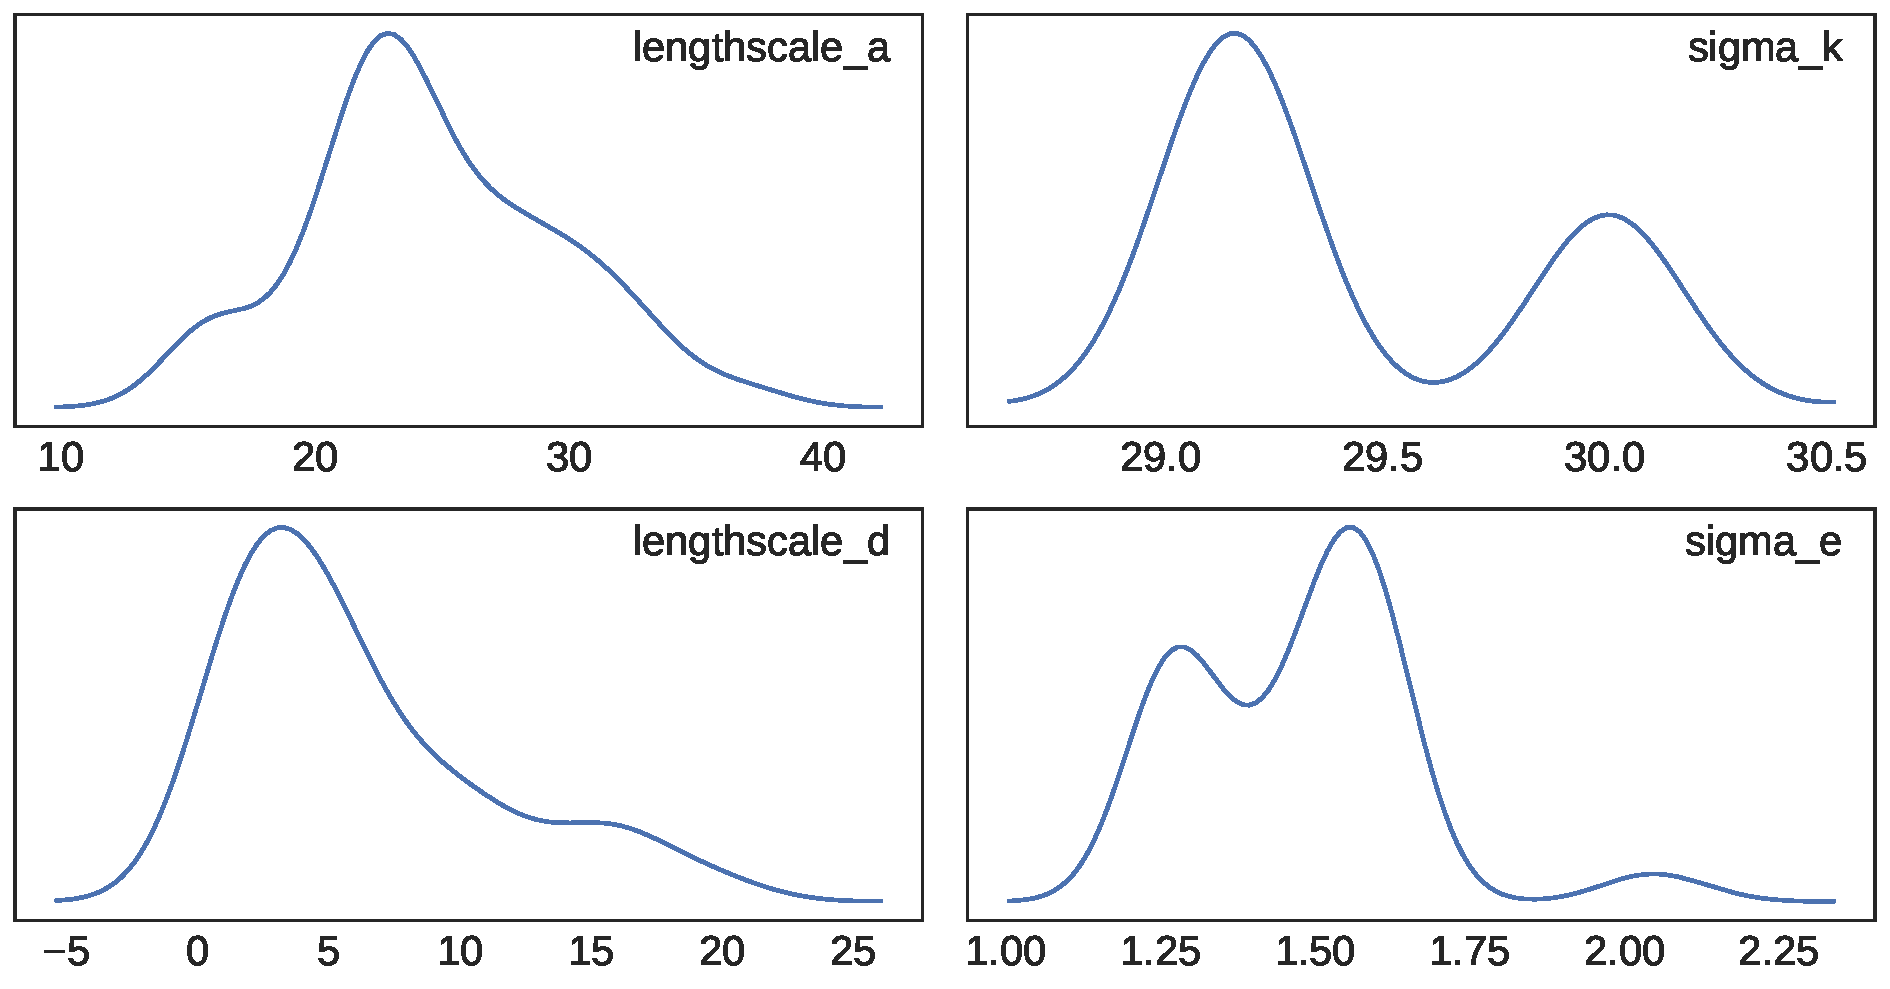
\includegraphics[width=0.5\textwidth]{img/fully_adaptive_hyperparameter_posteriors.pdf}
%	\caption{Posterior distributions after the final iteration sampling on fully-adaptive KAF experiment. $\sigma_k$ and $\sigma_e$ correspond to kernel and error parameters, while $l_\alpha$ and $l_s$ correspond to our prior parameters.}
%	\label{fig:fully-adaptive-posterior}
%\end{figure}

For the same wind data, we used a filter order $d=5$, a dictionary size of $10$, a forgetting factor $\rho=0.9$, a window length of $25$ samples, and $100$ MCMC samples per iteration to compute the MAP parameters. Fig. \ref{fig:adaptive-wind} shows the prediction of the proposed method trained online, where, in terms of MSE, the proposed fully-adaptive KAF implementation outperformed both the standard KLMS and the pre-trained KLMS (see the MSEs reported in Figs. \ref{wind-series} and \ref{fig:adaptive-wind}). This can be explained by the re-computation of the optimal parameters in each iteration, given a window of observations. The downside of this method is that computation time is considerable compared to standard KAF, mainly because the sampling stage of the algorithm requires compiling the log-posterior for every window before sampling even starts. We are currently improving this implementation for true online operation.

